Tacotron 2 merupakan penelitian yang diteliti oleh Google pada bulan Desember 2016. Tacotron-2 merupakan implementasi jaringan saraf untuk Text-to-Speech Synthesis. Silahkan kunjungi website https://google.github.io/tacotron/publications/tacotron2/ ini apabila teman-teman penasaran dengan penelitian tersebut. Apabila teman-teman perhatikan dan mencoba mendengarkan sampel suara yang ada di website tersebut bukankah sangat mirip dengan suara asli manusia? Setelah mendengarkan sampel suara tersebut saya menjadi sangat tertarik dengan penelitian tentang Arsitektur Tacotron-2 ini dan mencari tahu serta menerapkan model tersebut dalam project pembuatan voice cloning berbahasa indonesia ini. Cara kerja sistem dijelaskan oleh Jonathan Shen dan Ruoming Pang, Software Engineers, Google Brain and Machine Perception Teams.

''Singkatnya cara kerjanya seperti ini: Kami menggunakan model urutan-ke-urutan yang dioptimalkan untuk TTS untuk memetakan urutan huruf ke urutan fitur yang mengkodekan audio. Fitur-fitur ini, spektogram audio 80-dimensi dengan bingkai yang dihitung setiap 12,5 milidetik, tidak hanya menangkap pengucapan kata-kata, tetapi juga berbagai seluk-beluk ucapan manusia, termasuk volume, kecepatan, dan intonasi. Akhirnya fitur ini diubah menjadi bentuk gelombang 24 kHz menggunakan arsitektur mirip WaveNet."

\begin{figure}[H]
        \centerline{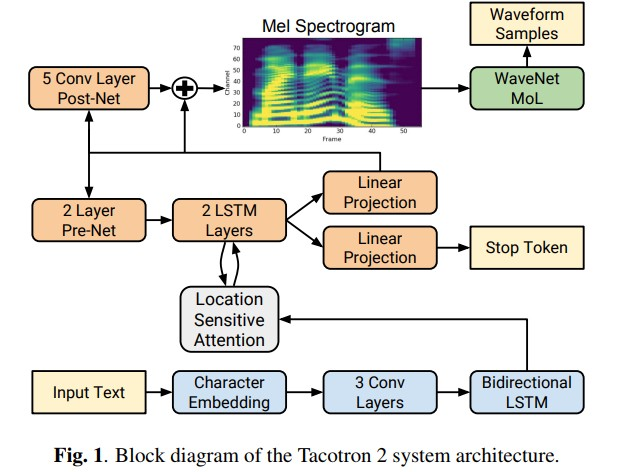
\includegraphics[scale=.75]{figures/fig1}}
        \caption{Blok Diagram dari Arsitektur Tacotron 2}
		\label{fig1}
\end{figure}

Bagian pertama dari model yaitu arsitektur Seq2Seq yang bertanggung jawab untuk mengubah teks menjadi mel-spektogram dan spektogram ini dimasukkan dalam model wave-net untuk menghasilkan bentuk gelombang audio. Satu hal yang menarik adalah kedua bagian dari arsitektur Tacotron (Seq2Seq dan vocoder Wavenet) ini dapat dilatih secara mandiri. Saya bekerja pada model Seq2Seq.
Modelnya adalah penyiapan enkoder-perhatian-dekoder di mana mereka menggunakan 'Perhatian sensitif lokasi'. Bagian pertama adalah Encoder yang mengubah urutan karakter menjadi vektor penyisipan kata. Representasi ini kemudian dikonsumsi oleh Decoder untuk memprediksi spektogram. Karena saya menggunakan dataset Indonesia, saya memastikan bahwa ruang karakter saya memiliki abjad Indonesia.

Encoder terdiri dari 3 lapisan konvolusi yang masing-masing berisi 512 filter berbentuk 5 x 1, diikuti oleh normalisasi batch dan aktivasi ReLU. Bagian selanjutnya adalah jaringan attention yang mengambil keluaran enkoder sebagai masukan dan mencoba meringkas urutan yang disandikan penuh sebagai vektor konteks dengan panjang yang tetap untuk setiap langkah keluaran dekoder.
Output dari lapisan konvolusi akhir dilewatkan ke lapisan LSTM dua arah tunggal yang berisi 512 unit (256 di setiap arah) untuk menghasilkan fitur yang dikodekan.

\section{MODEL BERBASIS PERHATIAN UNTUK PENGENALAN Pidato}
Mekanisme attention yang digunakan di sini memperhitungkan lokasi fokus pada langkah sebelumnya dan fitur urutan input.
Katakanlah kita memiliki data x = {x1,x2,x3….xN}. Kami meneruskan data ini ke encoder yang menghasilkan urutan keluaran yang dikodekan h = {h1,h2,h3….hN}.
A(i) = Perhatian( s(i-1), A(i-1), h ) di mana s(i-1) adalah status decoding sebelumnya dan A(i-1) adalah perataan sebelumnya.
s(i-1) adalah 0 untuk iterasi pertama dari langkah pertama.
Fungsi perhatian biasanya diimplementasikan dengan menilai setiap elemen dalam h secara terpisah dan kemudian menormalkan skor.
G(i) = A(i,0) h (0) + A(i,1) h (1) + ……. + A(i,N) h (N)
Y(i) ~ Hasilkan ( s(i-1), G(i) )
di mana s adalah output decoding, A(i) adalah vektor bobot perhatian yang disebut keselarasan.
Akhirnya, s(i) = Pengulangan ( s(i-1), G(i), Y(i) )
Pengulangan biasanya LSTM.

\subsection{Decoder}
Dekoder adalah jaringan saraf rekuren autoregresif yang memprediksi spektogram mel dari urutan input yang disandikan satu frame pada satu waktu. Prediksi dari langkah waktu sebelumnya pertama-tama dilewatkan melalui pra-net kecil yang berisi 2 lapisan yang terhubung penuh dari 256 unit ReLU tersembunyi. Output prenet dan vektor konteks perhatian digabungkan dan dilewatkan melalui tumpukan 2 lapisan LSTM uni-directional dengan 1024 unit. Akhirnya, spektogram mel yang diprediksi dilewatkan melalui post-net convolutional 5-lapisan yang memprediksi residu untuk ditambahkan ke prediksi untuk meningkatkan rekonstruksi keseluruhan. Setiap lapisan pasca jaring terdiri dari 512 filter dengan bentuk 5 × 1 dengan normalisasi batch, diikuti oleh aktivasi tanh pada semua kecuali lapisan terakhir.

\subsection{Loss Function}
Summed mean squared error (MSE)
Sejalan dengan prediksi bingkai spektogram, rangkaian keluaran LSTM dekoder dan konteks perhatian diproyeksikan ke skalar dan melewati aktivasi sigmoid untuk memprediksi kemungkinan bahwa urutan keluaran telah selesai. Prediksi "token berhenti" ini digunakan selama inferensi untuk memungkinkan model menentukan secara dinamis kapan harus menghentikan pembangkitan alih-alih selalu menghasilkan untuk durasi yang tetap.
Saya memutuskan untuk menggunakan pytorch untuk implementasi saya, melacak pelatihan dengan tensorboard , menggunakan GPU gcloud Tesla K80, terhubung ke port server dengan 'ssh -NfL', dan lab jupyter yang banyak digunakan selama pengembangan. [perlengkapan penyelamat hidup]
Saya mereferensikan berbagai repositori github [ 1 , 2 ] untuk memahami makalah, implementasi, mengoreksi bug dalam kode saya sendiri. Karena kompleksitas alami dari pernyataan masalah, saya tidak bisa mendapatkan hasil pidato yang menakjubkan seperti manusia tetapi saya belajar banyak hal tentang Text-to-speech dan itu adalah tujuan utama ketika saya mulai mengerjakan proyek ini.
Beberapa hasil untuk referensi:
\begin{figure}[H]
        \centerline{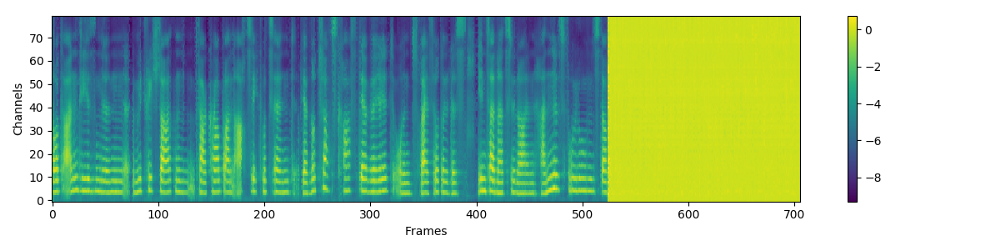
\includegraphics[scale=.75]{figures/ref1}}
        \caption{Spektogram mel yang diprediksi : Seperti yang dapat Anda bandingkan dengan wilayah atas, ia memiliki banyak celah dan masih membutuhkan banyak pelatihan. Sisi kanan (hijau solid) hanya padding dalam satu batch.}
		\label{ref1}
\end{figure}
\begin{figure}[H]
        \centerline{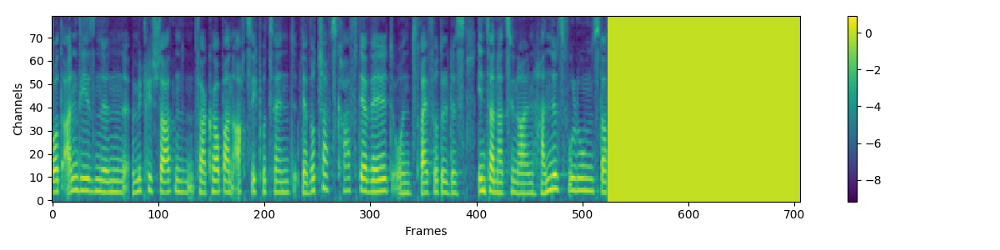
\includegraphics[scale=.75]{figures/ref2}}
        \caption{Target mel-spektogram}
		\label{ref2}
\end{figure}
\begin{figure}[H]
        \centerline{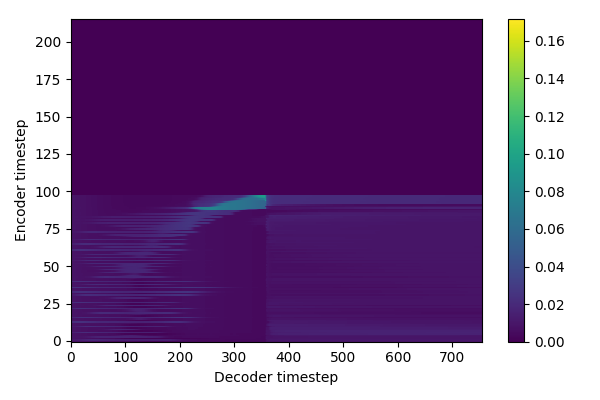
\includegraphics[scale=.75]{figures/ref3}}
        \caption{Perhatian (Seperti yang Anda lihat di sisi kiri bawah, sepertinya sedang belajar untuk menyelaraskan tetapi masih membutuhkan sekitar satu minggu pelatihan untuk mendapatkan diagonal yang sempurna untuk perhatian)}
		\label{ref3}
\end{figure}
Semua gambar yang dihasilkan di atas adalah setelah iterasi 50K (1 iterasi = 1 batch) yaitu 3 hari pelatihan. Model ini membutuhkan sekitar 300 ribu iterasi untuk mendekati seperti manusia. Anda dapat melihat bahwa, spektogram mel yang diprediksi terlihat cukup bagus bahkan ketika perhatian tidak dipelajari dengan benar. Selamatkan diri Anda dari jebakan dan pedulikan perhatian!

Menerapkan model dan pelatihan ternyata tidak sesepele yang saya kira awalnya. Saya menemukan banyak masalah yang saya ingin kalian ketahui sebelumnya dan menghemat waktu di GPU Anda.
Pelajari data Anda. Ini adalah bagian terpenting dari proyek. Dengarkan sampel data Anda, periksa panjang sampel teks, durasi sampel audio, dll. Anda dapat menghemat banyak waktu selama pelatihan, jika Anda mengetahui data Anda dengan baik. M-AILABS mengumumkan kumpulan data pidato besar mereka awal tahun ini. Mereka memiliki kumpulan data ucapan yang sangat banyak dalam berbagai bahasa. Saya menggunakan data Angela Merkel dari bagian wanita Jerman, yang memiliki 12 jam pidato dari pidato publik dan wawancaranya. Dataset ini lebih rendah dibandingkan dengan LJSpeech (dataset bahasa Inggris paling populer, 24 jam bicara). Saya menemukan ini hanya ketika saya mulai berlatih dan menghabiskan berhari-hari mengamati hasilnya. Jadi, bersiaplah!
TTS sangat mahal secara komputasi . Sebagai mahasiswa, saya baru saja memiliki akses ke satu GPU (Nvidia Tesla K80) di Google cloud. Mengingat struktur dataset yang saya gunakan, GPU saya hanya mengizinkan ukuran batch 8 saat pelatihan. Google mengatakan, mereka melatihnya dengan ukuran batch 64. Saya pertama kali mencoba dengan ukuran batch 2 (karena memori GPU terbatas) dan ketika model gagal menunjukkan konvergensi setelah 2-3 hari pelatihan, saya mengurutkan data saya sesuai panjang teks dan durasi audio, dan mulai berlatih dengan ukuran batch 8. Meskipun demikian, saya tidak dapat mengoptimalkan lebih banyak dengan dataset dan GPU yang saya miliki. Jadi, rencanakan dengan tepat.
Rasio pemaksaan guru. Dalam pelatihan paksa guru, model dibantu oleh label yang benar yaitu menggunakan kerangka Kebenaran Dasar saat ini untuk memprediksi langkah decoding berikutnya. Tidak jelas dalam makalah tentang rasio apa yang digunakan. Bahkan jika perhatiannya tidak dipelajari, model akan memprediksi kerangka yang baik untuk data pelatihan dalam mode paksaan guru tetapi dalam mode evaluasi itu tidak akan berhasil karena kita tidak memiliki kebenaran dasar (Mengira model itu bekerja sejak prediksi mels tampak bagus terlepas dari keberpihakan yang buruk). Saya melakukan pelatihan dengan 1.0, 0.75 dan 0.5 untuk membuat model belajar keberpihakan. Selama mode evaluasi, pemaksaan guru harus dimatikan.
Dibutuhkan berhari-hari untuk melatih dan mendapatkan keberpihakan. Ini adalah proses yang sangat rumit untuk melatih sistem TTS. Mungkin perlu sekitar 7–10 hari untuk melatih model asalkan Anda memiliki dukungan GPU terbatas (Kami bukan Google). Dan kemudian, men-debug kode dengan model seperti itu, adalah cerita lain.
Tuning hyperparameter adalah bagian yang sangat penting dari sistem Tacotron-2. Ukuran batch, tingkat pembelajaran, rasio guru-memaksa, panjang batch adalah beberapa parameter yang harus Anda perhatikan juga. Hal-hal bervariasi dengan dataset, jadi sangat sensitif!

Text-to-speech masih merupakan masalah penelitian yang sangat kompleks dan sangat menarik untuk dikerjakan. Pengalaman saya secara keseluruhan luar biasa dan saya belajar banyak hal tentang sistem TTS, bentuk gelombang audio, jaringan berulang, mel-spektogram, mekanisme perhatian dan saya harap posting ini dapat membantu Anda dalam perjalanan Anda dengan sistem TTS. Di masa mendatang, saya ingin melihat versi model Tacotron-2 yang dioptimalkan, sesuatu yang lebih kuat di berbagai bahasa, lebih mudah dilatih, dan tidak terlalu berat secara komputasi.
Jadi, saya hanya akan mengatakan, praproses data Anda dengan baik, sesuaikan hyperparameter Anda, catat semuanya di tensorboard dan mulai! Semua yang terbaik!